%%%%%%%%%%%%%%%%%%%%%%%%%%%%%%%%%%%%%%%%%
% baposter Portrait Poster
% LaTeX Template
% Version 1.0 (15/5/13)
%
% Created by:
% Brian Amberg (baposter@brian-amberg.de)
%
% This template has been downloaded from:
% http://www.LaTeXTemplates.com
%
% License:
% CC BY-NC-SA 3.0 (http://creativecommons.org/licenses/by-nc-sa/3.0/)
%
%%%%%%%%%%%%%%%%%%%%%%%%%%%%%%%%%%%%%%%%%

%----------------------------------------------------------------------------------------
%	PACKAGES AND OTHER DOCUMENT CONFIGURATIONS
%----------------------------------------------------------------------------------------

\documentclass[a0paper,portrait]{baposter}
\usepackage{cite,url,amsthm,footmisc,bm}
\usepackage{amsmath,graphicx,amssymb,algorithm,algorithmic,graphicx,subfigure,epsfig,multirow,threeparttable,booktabs,bm,mathdots,tabularx}
\usepackage[font=small,labelfont=bf]{caption} % Required for specifying captions to tables and figures
\usepackage{booktabs} % Horizontal rules in tables
\usepackage{relsize} % Used for making text smaller in some places

\graphicspath{{figures/}} % Directory in which figures are stored

\definecolor{bordercol}{RGB}{40,40,40} % Border color of content boxes
\definecolor{headercol1}{RGB}{186,215,230} % Background color for the header in the content boxes (left side)
\definecolor{headercol2}{RGB}{80,80,80} % Background color for the header in the content boxes (right side)
\definecolor{headerfontcol}{RGB}{256,256,256} % Text color for the header text in the content boxes
\definecolor{boxcolor}{RGB}{256,256,256} % Background color for the content in the content boxes

\begin{document}

\background{ % Set the background to an image (background.pdf)
\begin{tikzpicture}[remember picture,overlay]
\draw (current page.north west)+(-2em,2em) node[anchor=north west]
{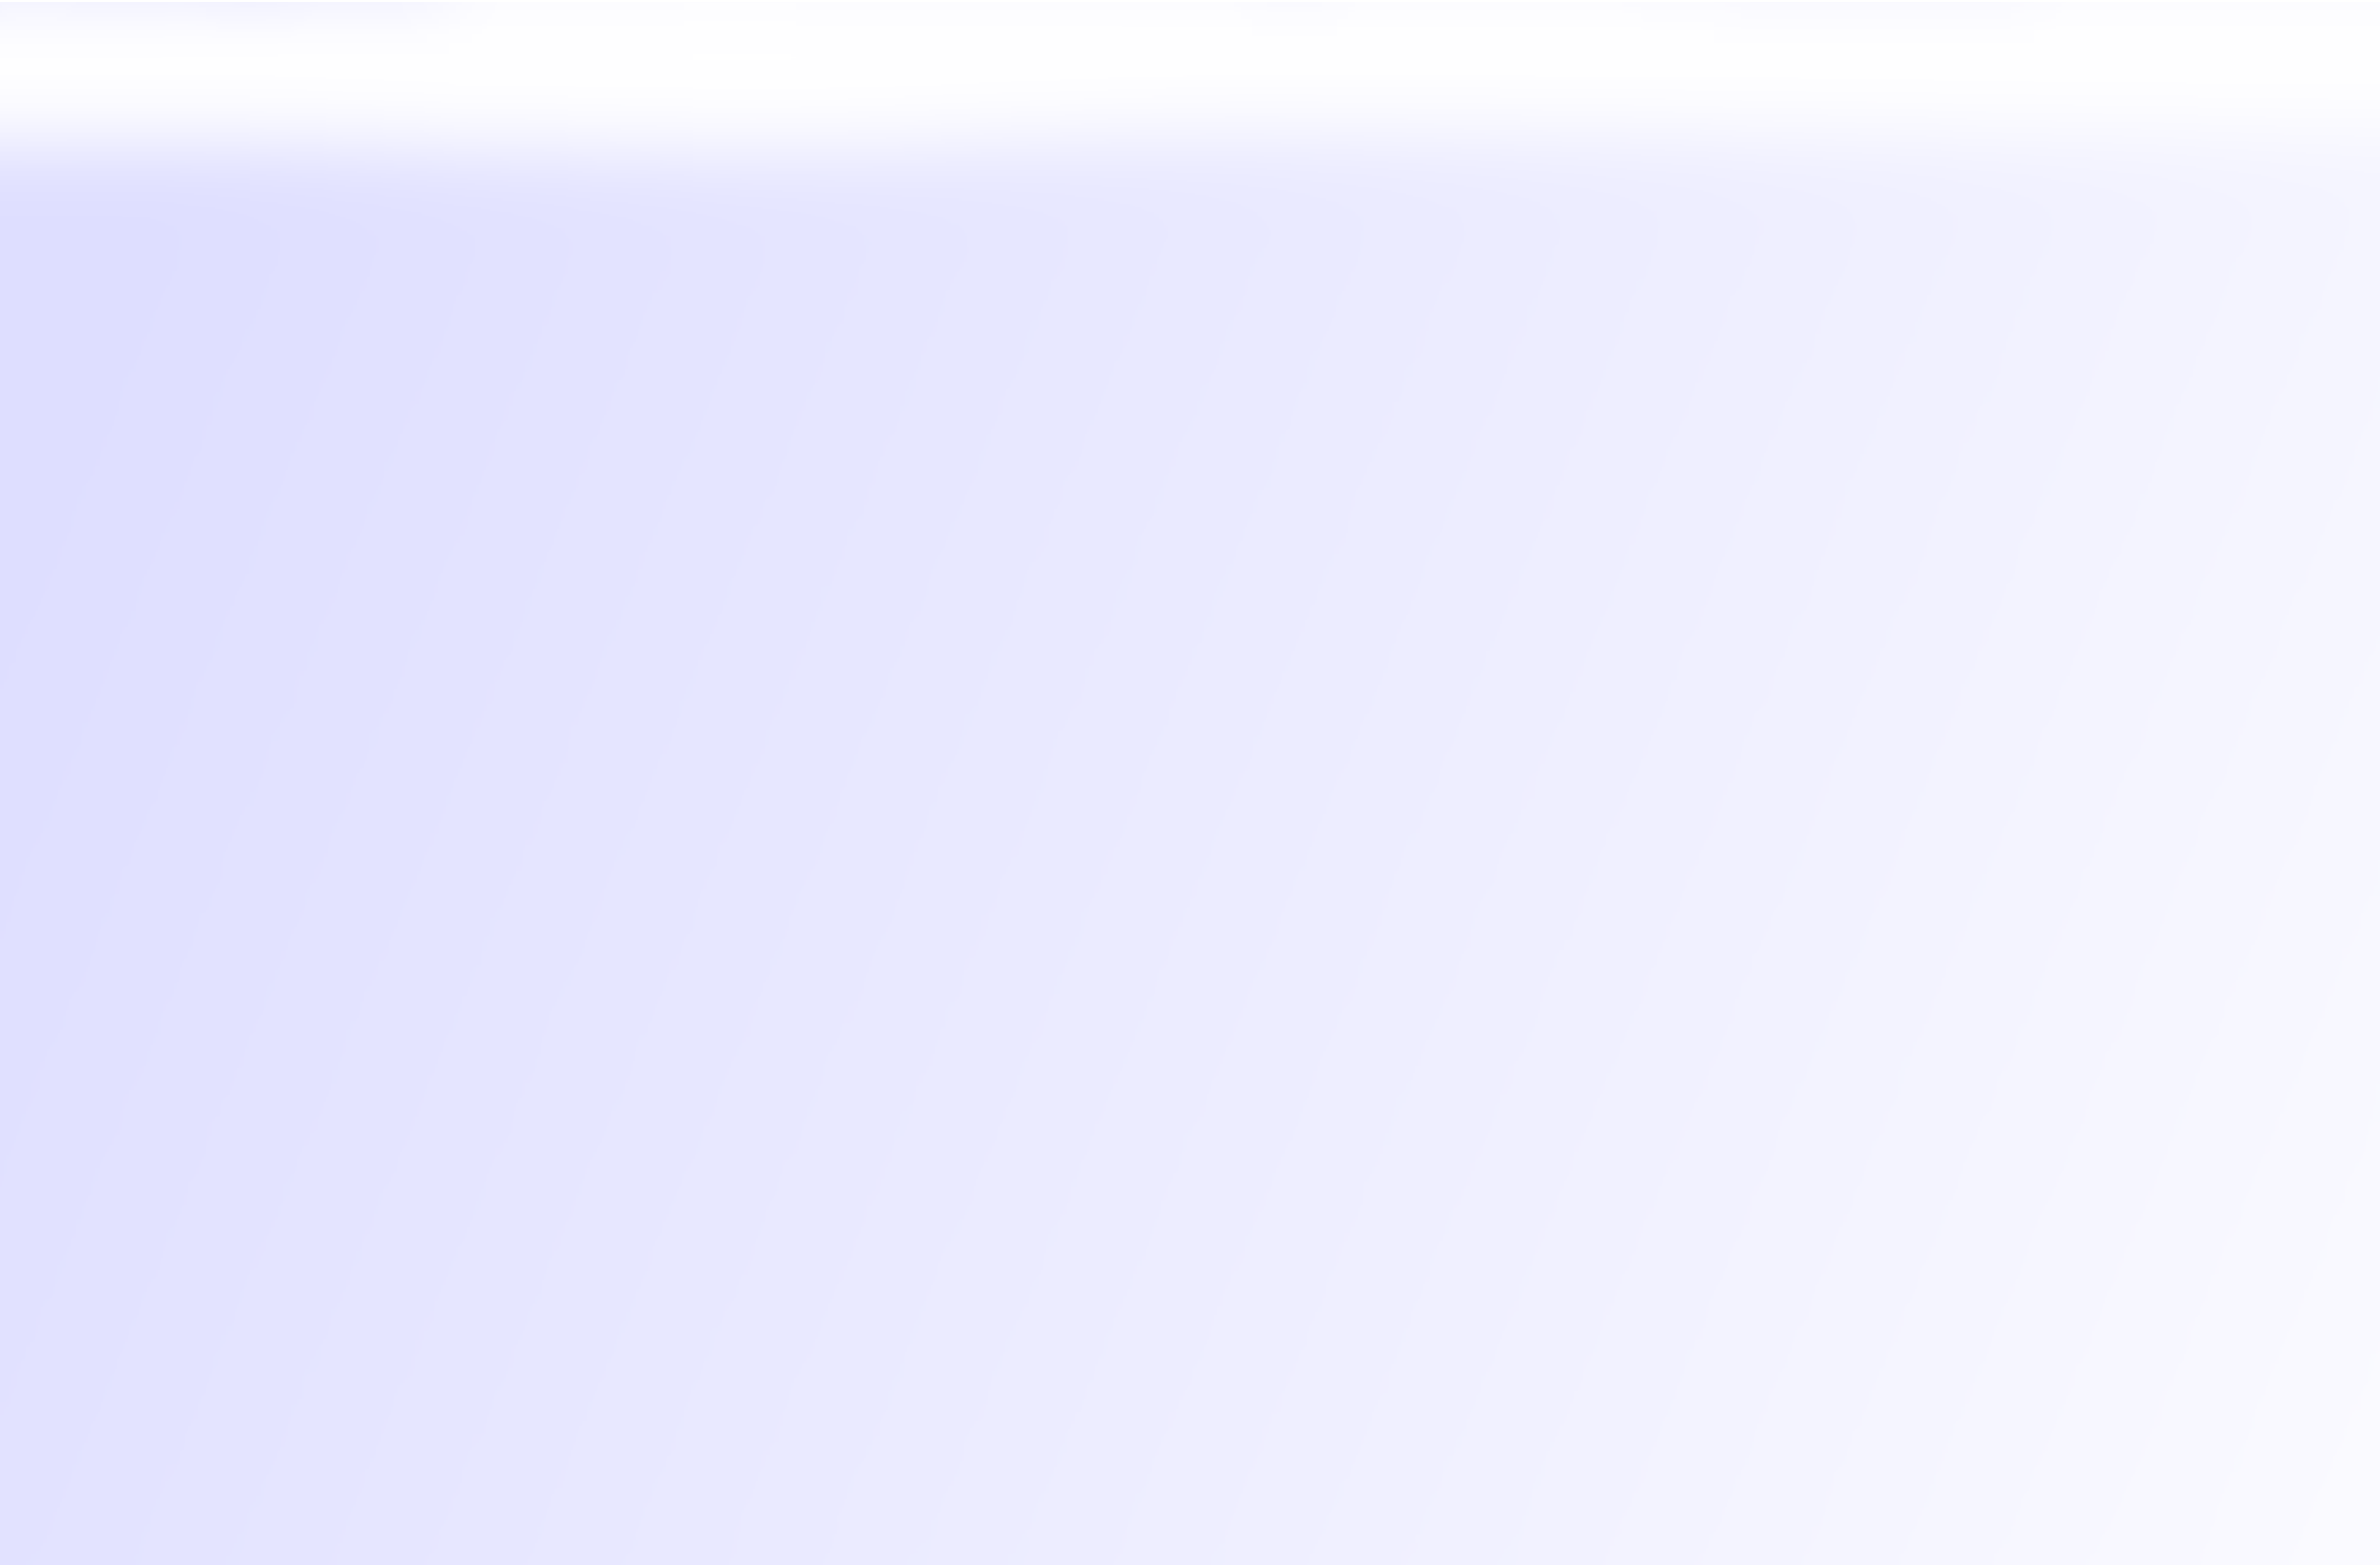
\includegraphics[height=1.1\textheight]{background}};
\end{tikzpicture}
}

\begin{poster}{
grid=false,
borderColor=bordercol, % Border color of content boxes
headerColorOne=headercol2, % Background color for the header in the content boxes (left side)
headerColorTwo=headercol1, % Background color for the header in the content boxes (right side)
headerFontColor=headerfontcol, % Text color for the header text in the content boxes
boxColorOne=boxcolor, % Background color for the content in the content boxes
headershape=roundedright, % Specify the rounded corner in the content box headers
headerfont=\Large\sf\bf, % Font modifiers for the text in the content box headers
textborder=rectangle,
background=user,
headerborder=open, % Change to closed for a line under the content box headers
boxshade=plain
}
{}
%
%----------------------------------------------------------------------------------------
%	TITLE AND AUTHOR NAME
%----------------------------------------------------------------------------------------
%
{\bf JOINT STRUCTURED GRAPH LEARNING AND UNSUPERVISED FEATURE SELECTION} % Poster title
{\vspace{1em} Yong Peng, Leijie Zhang, Wanzeng Kong, Feiping Nie and Andrzej Cichocki\\ % Author names
{\smaller yongpeng@hdu.edu.cn}} % Author email addresses
{
\includegraphics[scale=1.55]{logo}} % University/lab logo

%----------------------------------------------------------------------------------------
%	INTRODUCTION
%----------------------------------------------------------------------------------------

\headerbox{Abstract}{name=introduction,column=0,row=0}{

The central task in graph-based unsupervised feature selection (GUFS) depends on two folds, one is to accurately characterize the geometrical structure of the original feature space with a graph and the other is to make the selected features well preserve such intrinsic structure. Currently, most of the existing GUFS methods use a two-stage strategy which constructs graph first and then perform feature selection on this fixed graph. Since the performance of feature selection severely depends on the quality of graph, the selection results will be unsatisfactory if the given graph is of low-quality. To this end, we propose a joint graph learning and unsupervised feature selection (JGUFS) model in which the graph can be adjusted to adapt the feature selection process. The JGUFS objective function is optimized by an efficient iterative algorithm whose convergence and complexity are analyzed in detail. Experimental results on representative benchmark data sets demonstrate the improved performance of JGUFS in comparison with state-of-the-art methods and therefore we conclude that it is promising of allowing the feature selection process to change the data graph.
}

%----------------------------------------------------------------------------------------
%	MATERIALS AND METHODS
%----------------------------------------------------------------------------------------

\headerbox{Model Formulation}{name=methods,column=0,below=introduction}{

\begin{equation}
\begin{aligned}
\min_{\mathbf{S},\mathbf{W},\mathbf{F}}&\|\mathbf{S}-\mathbf{A}\|_F^2+\alpha\mathbf{Tr}(\mathbf{F}^T\mathbf{L_s}\mathbf{F})+\\&\beta(\|(\mathbf{XW}-\mathbf{F}\|_F^2+\gamma\|\mathbf{W}\|_{2,1}) \\
s.t.&~\mathbf{S1}=\mathbf{1},\mathbf{S}\ge\mathbf{0},\mathbf{F}^T\mathbf{F}=\mathbf{I}_c,\mathbf{F}\ge\mathbf{0}
\end{aligned}
\label{eq:3}
\end{equation}
where $\mathbf{X}\in\mathbb{R}^{n\times d}$ is the data matrix, $\mathbf{W}\in\mathbb{R}^{d\times c}$ is the projection matrix, $\beta$ and $\gamma$ are regularization parameters. Similar to [1, 2], we impose the non-negativity on F here
}

%----------------------------------------------------------------------------------------
%	CONCLUSION
%----------------------------------------------------------------------------------------

\headerbox{Conclusion}{name=conclusion,column=0,below=methods}{

In this paper, we proposed a novel GUFS method, termed JGUFS, which simultaneously performs graph construction and feature selection. Instead of performing feature selection on a fixed graph, JGUFS successfully avoided the disadvantages caused by the two-stage strategy. In JGUFS, the subobjectives respectively corresponding to graph construction and unsupervised feature selection could co-evolve towards the optimum. An efficient iterative optimization method with convergence guarantee was presented to optimize the JGUFS objective. Extensive experiments were conducted on representative data sets to demonstrate the excellent performance of JGUFS in comparison with state-of-the-art methods.
}

%----------------------------------------------------------------------------------------
%	REFERENCES
%----------------------------------------------------------------------------------------

\headerbox{References}{name=references,column=0,below=conclusion}{

\smaller % Reduce the font size in this block
\renewcommand{\section}[2]{\vskip 0.05em} % Get rid of the default "References" section title
\nocite{*} % Insert publications even if they are not cited in the poster

\bibliographystyle{unsrt}
\bibliography{sample} % Use sample.bib as the bibliography file
}

%----------------------------------------------------------------------------------------
%	ACKNOWLEDGEMENTS
%----------------------------------------------------------------------------------------



%----------------------------------------------------------------------------------------
%	RESULTS 1
%----------------------------------------------------------------------------------------

\headerbox{Performance in Feature Selection}{name=results1,span=2,column=1,row=0}{ % To reduce this block to 1 column width, remove 'span=2'
\vspace{-15pt}
 \begin{table}[H]
  \centering
  \caption{Comparison of  of clustering for different feature selection methods (ACC/NMI$\pm$std).}
  \vspace{-5pt}
  \begin{tabular}{|c|c|c|c|c|c|c|c|} \hline
  $\mathbf{ACC}$ & JAFFE & UMIST & USPS & MNIST & COIL20   & WebKB & ISOLET \\ \hline
	All-Fea &72.1$\pm$3.3 &42.9$\pm$2.8 &63.7$\pm$4.1 &51.8$\pm$4.7 &61.7$\pm$2.4 &55.9$\pm$3.1 &57.4$\pm$3.9\\ \hline
	MaxVar &76.3$\pm$2.9 &46.7$\pm$2.4 &64.9$\pm$3.1 &53.0$\pm$2.9 &61.1$\pm$2.8 &54.8$\pm$2.3 &56.9$\pm$2.7\\ \hline
	LapScore &77.2$\pm$3.2 &45.8$\pm$3.0 &64.1$\pm$3.2 &53.9$\pm$3.5 &62.1$\pm$2.1 &56.1$\pm$2.8 &56.8$\pm$2.9\\ \hline
	MCFS &79.5$\pm$2.7 &46.7$\pm$3.1 &65.1$\pm$4.7 &55.9$\pm$3.7 &60.9$\pm$2.3 &61.5$\pm$2.3 &60.9$\pm$2.5\\ \hline
	FSSL &85.6$\pm$2.2 &51.9$\pm$3.3 &66.5$\pm$2.4 &57.1$\pm$3.8 &62.5$\pm$2.8 &62.3$\pm$2.7 &64.9$\pm$3.1\\ \hline
	UDFS &84.7$\pm$2.3 &48.9$\pm$3.8 &66.3$\pm$3.0 &56.7$\pm$3.2 &60.8$\pm$2.7 &61.9$\pm$2.9 &64.7$\pm$3.6\\ \hline
	NDFS &86.9$\pm$2.5 &51.1$\pm$3.7 &66.9$\pm$2.7 &58.5$\pm$2.8 &63.3$\pm$2.1 &62.5$\pm$3.0 &65.1$\pm$3.9\\ \hline
	JELSR &86.5$\pm$2.3 &53.7$\pm$3.2 &67.8$\pm$2.9 &58.1$\pm$3.1 &64.8$\pm$1.9 &61.8$\pm$2.9 &63.7$\pm$2.8\\ \hline
	JGUFS &88.3$\pm$2.4 &57.8$\pm$2.6 &69.7$\pm$2.8 &59.3$\pm$3.0 &68.9$\pm$1.6 &63.8$\pm$2.7 &66.8$\pm$3.2 \\\hline \hline
    $\mathbf{NMI}$ &JAFFE &UMIST &USPS &MNIST &COIL20 &WebKB &ISOLET\\ \hline
	All-Fea &78.9$\pm$2.1 &63.5$\pm$2.2 &59.7$\pm$1.8 &46.3$\pm$2.1 &73.5$\pm$2.8 &11.7$\pm$4.2 &73.9$\pm$1.7\\ \hline
	MaxVar &80.3$\pm$2.0 &65.1$\pm$2.0 &60.9$\pm$1.5 &47.9$\pm$2.3 &71.8$\pm$3.1 &16.9$\pm$2.1 &73.7$\pm$1.8\\ \hline
	LapScore &81.9$\pm$1.8 &64.7$\pm$2.6 &60.3$\pm$1.3 &48.3$\pm$2.0 &73.9$\pm$2.9 &13.4$\pm$3.5 &72.1$\pm$1.1\\ \hline
	MCFS &82.3$\pm$1.8 &65.6$\pm$1.8 &61.7$\pm$1.5 &50.3$\pm$1.7 &74.8$\pm$2.3 &18.3$\pm$3.7 &74.9$\pm$1.6\\ \hline
	FSSL &88.6$\pm$1.3 &67.7$\pm$2.0 &62.3$\pm$1.3 &50.8$\pm$2.1 &75.1$\pm$2.7 &18.5$\pm$3.5 &76.8$\pm$1.7\\ \hline
	UDFS &85.3$\pm$2.0 &66.5$\pm$2.1 &61.8$\pm$1.5 &50.1$\pm$1.5 &75.7$\pm$1.9 &17.1$\pm$2.9 &76.3$\pm$1.9\\ \hline
	NDFS &87.6$\pm$1.9 &68.9$\pm$2.5 &61.3$\pm$1.1 &51.6$\pm$1.1 &77.3$\pm$1.8 &17.6$\pm$2.7 &78.4$\pm$1.2\\ \hline
	JELSR &86.9$\pm$2.1 &70.3$\pm$1.7 &62.0$\pm$1.3 &51.1$\pm$1.4 &77.9$\pm$1.7 &18.0$\pm$3.1 &75.8$\pm$1.1\\ \hline
	JGUFS &89.8$\pm$0.6 &73.9$\pm$2.1 &63.9$\pm$1.1 &52.9$\pm$1.0 &79.8$\pm$1.3 &20.3$\pm$2.3 &79.9$\pm$1.2\\ \hline
  \end{tabular}
  \label{tab:results}
\end{table}

}

%----------------------------------------------------------------------------------------
%	RESULTS 2
%----------------------------------------------------------------------------------------

\headerbox{Optimization}{name=results2,span=1,column=1,below=results1,above=bottom}{ % To reduce this block to 1 column width, remove 'span=2'
With other two variables fixed, the following formula can be proved: 
\begin{equation}\nonumber
\begin{aligned}
&\mathcal{O}(\mathbf{F}^{t+1}, \mathbf{W}^{t},\mathbf{S}^{t}) \leq \mathcal{O}(\mathbf{F}^{t}, \mathbf{W}^{t},\mathbf{S}^{t}), \\ &\mathcal{O}(\mathbf{F}^{t+1}, \mathbf{W}^{t+1},\mathbf{S}^{t}) \leq \mathcal{O}(\mathbf{F}^{t+1}, \mathbf{W}^{t},\mathbf{S}^{t}) \\ &\mathcal{O}(\mathbf{F}^{t+1}, \mathbf{W}^{t+1},\mathbf{S}^{t+1}) \leq \mathcal{O}(\mathbf{F}^{t+1}, \mathbf{W}^{t+1},\mathbf{S}^{t})
\end{aligned}
\end{equation}

We conclude that JGUFS objective function monotonically decreases under the optimization in Algorithm. 1.

\begin{algorithm}[H]
  \renewcommand{\algorithmicrequire}{\textbf{Input:}}
  \renewcommand{\algorithmicensure}{\textbf{Output:}}
  \caption{Optimization to JGUFS objective function}
    \begin{algorithmic}[1]
    \REQUIRE Data matrix $\mathbf{X}\in\mathbb{R}^{n\times d}$, $\lambda$, $\beta$, and $\gamma$, $c$, the dimension of projected subspace c;
    \ENSURE Rank features based on the values of $\|w_i\|_2|_{i=1}^d$ in descending order and then select the top-ranked ones.
    \STATE Initialization. Construct the initial graph affinity matrix $\mathbf{A}$ based on the 'HeatKernel' function; Calculate $\mathbf{F}\in\mathbb{R}^{n\times c}$ by the c eigenvectors of the graph Laplacian $\mathbf{L_A}=\mathbf{D_A}-\frac{\mathbf{A}^T+\mathbf{A}}{2}$ corresponding to the c smallest eigenvalues; Initialize $\mathbf{M}\in\mathbb{R}^{d\times d}$ as an identity matrix;;
    \WHILE {not converged}
    \STATE Update $\mathbf{S}$ by solving:
    \vspace{-10pt}
    \begin{equation}\nonumber
        \min_{S_i\mathbf{1}=1,s_i\ge0}\|s_i-(a_i-\frac{\alpha}{2}d_i)\|_F^2,
    \end{equation}
    
    where, $d_{ij}=\|f_i-f_j\|_2^2$ and $d_i$ as a vector with the $j$-th element equal to $d_{ij}$. Similarly, we get $a_i$ and $s_i$.
    \STATE Update $\mathbf{W}$ by:
    \vspace{-7pt}
    \begin{equation}\nonumber
       \mathbf{W}=(\mathbf{X}^T\mathbf{X}+\gamma\mathbf{M})^{-1}\mathbf{X}^T\mathbf{F}
    \end{equation}
    \vspace{-15pt}
    \STATE Update $\mathbf{M}$ by:
    \vspace{-7pt}
    \begin{equation}\nonumber
        m_{ii}=\frac{1}{2\|w\|_2}=\frac{1}{2\sqrt{w_iw_i^T+\delta}}
    \end{equation}
    \vspace{-10pt}
    \STATE Update $\mathbf{F}$ by:
    \vspace{-10pt}
    \begin{equation}\nonumber
        d_{ij} \leftarrow \frac{(\lambda \mathbf{F})_{ij}}{\mathbf{R}\mathbf{F}+\lambda\mathbf{FF}^T\mathbf{F}}
    \end{equation}
    \vspace{-15pt}
    \ENDWHILE
    \end{algorithmic}
    \label{alg:1}
\end{algorithm}

%------------------------------------------------

}

%----------------------------------------------------------------------------------------
---
%	RESULTS 2
%----------------------------------------------------------------------------------------

\headerbox{Analysis}{name=results2,span=1,column=2,below=results1,above=bottom}{ % To reduce this block to 1 column width, remove 'span=2'
Figure 1 illustrates the clustering performance of JGUFS on COIL20 with different settings of parameters. From this figure, we find that JGUFS provides excellent performance when the parameters are set as different values in a wide range. Further, we can observe that even if a small number of features are selected, JGUFS can still achieve relatively good clustering results.

\vspace{-5pt}
%------------------------------------------------

\begin{center}
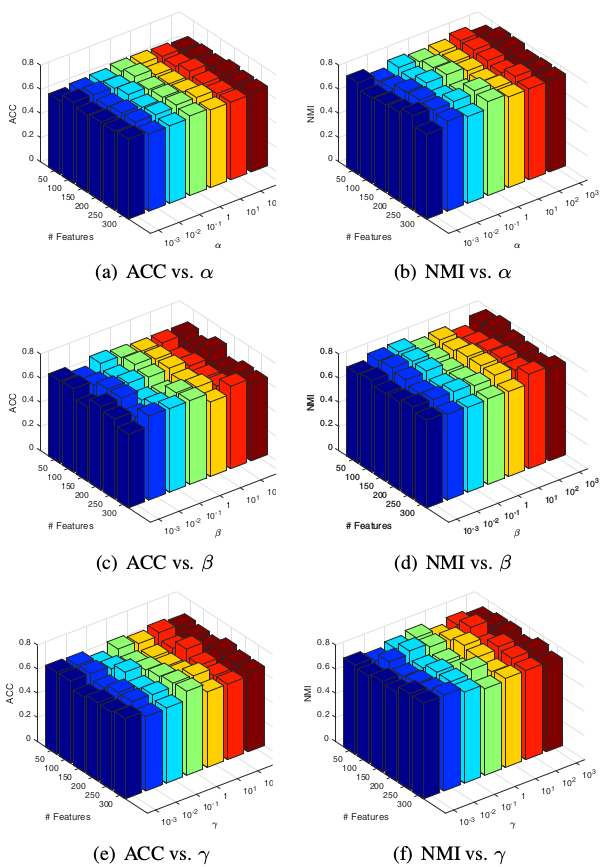
\includegraphics[width=0.8\linewidth]{result_bar.jpg}
\vspace{-8pt}
\captionof{figure}{Performance of JGUFS algorithm for large variation of set of control parameters.}
\end{center}

%------------------------------------------------
\vspace{-15pt}
\begin{center}
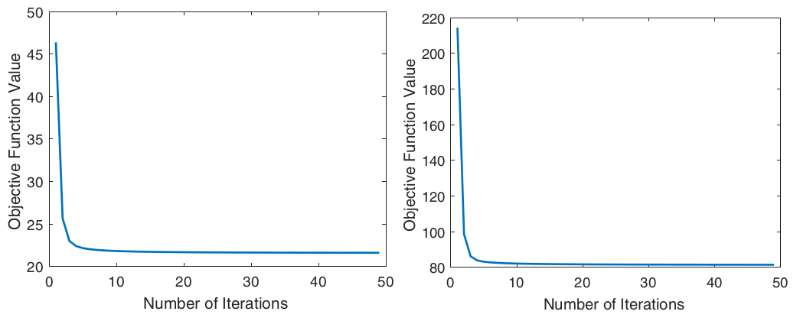
\includegraphics[width=0.8\linewidth]{result_cur.jpg}
\vspace{-8pt}
\captionof{figure}{Convergence speed of JGUFS for UMIST and COIL20 data sets.}
\end{center}

%------------------------------------------------
\vspace{-8pt}
 Figure 2 shows the convergence curves of the JGUFS objective function in terms of the number of iterations on UMIST and COIL20 from which we can observe that JGUFS has a relatively fast convergence speed. 


}

\end{poster}

\end{document}